% ===================== TMD correlator for lattice calculations (thesis Ch. 4) =====================
\section{TMD correlator}

% Slide 14
\begin{frame}{Definition of TMDs}
  \begin{itemize}
    \item Nucleon with $P^+\gg\mN$, $\vprp P=0$: $x=k^+/P^+$ and $\vprp k$ are boost invariant along $z$.
    \item Gauge-invariant bilocal operator, divided by the soft factor $\widetilde{\softf}$ (rapidity divergences). Wilson-line geometry, rapidity-regulator and renormalization-scale arguments are held fixed and suppressed below:
  \end{itemize}
  \[ \Phi^{[\Gamma]}(\kei,P,S)\equiv\int \frac{d^4 \bvec}{(2\pi)^4}\, e^{i \kei\cdot \bvec}\,
     \frac{\overbrace{\tfrac{1}{2}\, \bra{P,S}\ \bar{q}(0)\, \Gamma\ \WlineC{\mathcal{C}_\bvec}\ q(\bvec)\ \ket{P,S}}^{\textstyle \equiv\ \widetilde \Phi_\unsub^{[\Gamma]}(\bvec,P,S)}}{\widetilde{\softf}(\bvec^2)} \]
  \begin{itemize}
    \item Integrating over $k^-$ sets $\bvec^+=0$:
  \end{itemize}
  \[ \Phi^{[\Gamma]}(x,\vprp{k};P,S)=\int \frac{d^2 \vprp{\bvec}}{(2\pi)^2} \int \frac{d (\bvec \tcdot P)}{(2\pi) P^+}\ e^{i x (\bvec \tcdot P) - i\vprp{\bvec} \tcdot \vprp{\kei}}\,\frac{\widetilde \Phi_\unsub^{[\Gamma]}}{\widetilde{\softf}}\Big|_{\bvec^+=0} \]
  \keymsg{$x \leftrightarrow \bvec \tcdot P$ \ and \ $\vprp{k} \leftrightarrow \vprp{b}$ are Fourier pairs. \qquad
  $\Phi^{[\gamma^+]} = f_1 - \dfrac{\myeps_{ij}\, k_{i}\, S_{j}}{\mN}\ f_{1T}^\prp$}
\end{frame}

% Slide 15
\begin{frame}{TMDs in Fourier space}
  \begin{itemize}
    \item The lattice computes $\bvec$-space matrix elements, so we state results for $\vprp b$-dependent TMDs:
  \end{itemize}
  \[ \tilde f(x, \vprp{\bvec}^2) \equiv \int  d^2 \vprp{\kei} \, e^{i \vprp{\bvec} \cdot \vprp{\kei} }\, f(x, \vprp{\kei}^2)
     = 2\pi \int d|\vprp{\kei}|\, |\vprp{\kei}|\ J_0(|\vprp{\bvec}||\vprp{\kei}|)\  f(x, \vprp{\kei}^2) \]
  \[ \tilde f^{(n)}(x, \vprp{\bvec}^2) \equiv n!\left( -\frac{2}{\mN^2}\partial_{\vprp{\bvec}^2} \right)^n \tilde f(x, \vprp{\bvec}^2)
     \ \xrightarrow{\ |\vprp b|\to0\ }\ \int  d^2 \vprp{\kei} \left( \frac{\vprp{\kei}^2}{2 \mN^2 }\right)^n  f(x, \vprp{\kei}^2) \]
  \begin{itemize}
    \item $\tilde f_1^{(0)}$: unpolarized; \ $\tilde f_{1T}^{\perp(1)}$: first $\vprp k$-moment of the Sivers function.
    \item $f_{1T}^{\perp(1)}(x)$ diverges without extra regularization (high-$\vprp k$ tail), so we \textbf{stay at finite $|\vprp b|$}.
    \item Finite $|\vprp b|$ provides Bessel weighting. The correlator still requires ultraviolet and rapidity renormalization. We reach $x$ through $\bvec\tcdot P$.
  \end{itemize}
\end{frame}

% Slide 16
\begin{frame}{Link geometry}
  \begin{columns}[c]
    \begin{column}{0.55\textwidth}
      \begin{itemize}
        \item Staple-shaped link $\mathcal U[0,\eta v,\eta v+\bvec,\bvec]$: legs along $v$ of length $\eta|v|$, joined at the far end.
        \item Large staple extent: SIDIS for $\eta v\tcdot P\to+\infty$ and Drell--Yan for $\eta v\tcdot P\to-\infty$.
        \item On the lattice $\bvec$ and $v$ are purely spatial (space-like). Collins--Soper parameter:
      \end{itemize}
      \[ \zetahat \equiv \frac{\zeta}{2\mN}=\frac{v \cdot P}{\sqrt{|v^2|}\, \sqrt{P^2}} = \sinh(y_P - y_v) \]
      \begin{itemize}
        \item Light-like $v$ (the TMD limit) $\Leftrightarrow$ $\zetahat\to\infty$.
      \end{itemize}
    \end{column}
    \begin{column}{0.43\textwidth}
      \centering
      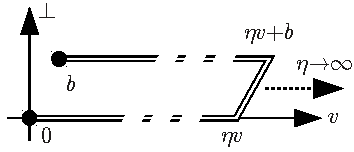
\includegraphics[width=\linewidth]{StapleLink2.pdf}
    \end{column}
  \end{columns}
\end{frame}

% Slide 17
\begin{frame}{Symmetry constraints: the amplitudes are complex}
  \begin{itemize}
    \item The correlator is decomposed into Lorentz-invariant amplitudes ($A_i$, $B_i$ in momentum space; $\tAmp_i$, $\tBmp_i$ in $\bvec$-space; next slide). Lorentz, parity, time reversal and Hermiticity constrain it; in momentum space Hermiticity makes $A_i$, $B_i$ \textbf{real}.
    \item In $\bvec$-space ($\kei\to -i\mN^2\bvec$), Hermitian conjugation gives
  \end{itemize}
  \[ \big[\widetilde{\Phi}^{[\GammaOp]}_{\unsub}(\bvec,P,S;v)\big]^* = \widetilde{\Phi}^{[\gamma^0 \GammaOp^\dagger \gamma^0]}_{\unsub}(-\bvec,P,S;v) \]
  \[ \Rightarrow\quad \big[\tAmp_i(\bvec^2,\bvec \tcdot P, \tfrac{v \tcdot \bvec}{v \tcdot P}, \zeta^{-2})\big]^* = \tAmp_i(\bvec^2,-\bvec \tcdot P, -\tfrac{v \tcdot \bvec}{v \tcdot P}, \zeta^{-2}) \]
  \keymsg{$\tAmp_i=\tAmp_i^{\text{Re}}+i\tAmp_i^{\text{Im}}$ \ are complex, with \ $\tAmp_i^{\text{Re}}$: even in $\bvec$, \quad $\tAmp_i^{\text{Im}}$: odd in $\bvec$ \quad (same for $\tBmp_i$)}
\end{frame}

% Full vector decomposition, with no suppressed tensor structures.
\begin{frame}{Complete vector-correlator decomposition}
  \small
  \begin{align*}
  \frac12\widetilde\Phi_{\unsub}^{[\gamma^\mu]}
   ={}&P^\mu\tAmp_2-i\mN^2 b^\mu\tAmp_3
       -i\mN\epsilon^{\mu\nu\alpha\beta}P_\nu b_\alpha S_\beta\tAmp_{12}\\
   &+\frac{\mN^2}{v\cdot P}v^\mu\tBmp_1
       +\frac{\mN}{v\cdot P}\epsilon^{\mu\nu\alpha\beta}P_\nu v_\alpha S_\beta\tBmp_7\\
   &-\frac{i\mN^3}{v\cdot P}\epsilon^{\mu\nu\alpha\beta}b_\nu v_\alpha S_\beta\tBmp_8\\
   &-\frac{\mN^3}{v\cdot P}(b\cdot S)\epsilon^{\mu\nu\alpha\beta}P_\nu b_\alpha v_\beta\tBmp_9\\
   &-\frac{i\mN^3}{(v\cdot P)^2}(v\cdot S)\epsilon^{\mu\nu\alpha\beta}P_\nu b_\alpha v_\beta\tBmp_{10}.
  \end{align*}
  \begin{itemize}
    \item All eight allowed structures of this vector channel are retained.
    \item Each amplitude is a function of
    $\big(b\cdot b,\ b\cdot P,\ (v\cdot b)/(v\cdot P),\ -1/(\mN\zetahat)^2,\ \eta v\cdot P\big)$.
    \item Here $b\cdot b$ is the Minkowski square. A spatial component $b^2$ later denotes the second component, not this invariant.
  \end{itemize}
  \figsrc{Thesis, TMD framework, vector parametrization; Musch et al., Phys. Rev. D 85, 094510 (2012).}
\end{frame}

\begin{frame}{The two amplitude combinations entering the Sivers shift}
  In the TMD frame, $b^+=0$ and $\vprp v=\vprp P=0$ fix the third invariant:
  \[
  \frac{v\cdot b}{v\cdot P}=(b\cdot P)\frac{R(\zetahat^2)}{\mN^2},
  \qquad R(\zetahat^2)=1-\sqrt{1+\zetahat^{-2}}.
  \]
  The $\gamma^+$ projection becomes
  \[
  \frac{1}{2P^+}\widetilde\Phi_{\unsub}^{[\gamma^+]}
  =\tAmp_{2B}+i\mN\epsilon_{ij}\vect b_i\vect S_j\tAmp_{12B}.
  \]
  \[
    \boxed{\tAmp_{2B}=\tAmp_2+R(\zetahat^2)\tBmp_1},
    \qquad
    \boxed{\tAmp_{12B}=\tAmp_{12}-R(\zetahat^2)\tBmp_8}.
  \]
  \begin{itemize}
    \item These combinations follow from the full vector decomposition.
    \item We determine them from the four Euclidean vector channels, after path averaging and interpolation.
  \end{itemize}
  \figsrc{Thesis, TMD framework, TMD-frame reduction; Musch et al. (2012).}
\end{frame}

% Slide 19
\begin{frame}{Generalized Sivers shift from amplitudes}
  \begin{itemize}
    \item Average $k_y$ of unpolarized quarks in a nucleon polarized along $\hat x$ ($T$: transversely polarized nucleon, $U$: unpolarized quark), generalized to finite $|\vprp b|$:
  \end{itemize}
  \begin{block}{}
  \[ \langle k_y\rangle_{TU}(\vprp{b}^2;\zetahat,\eta v\tcdot P) \equiv \mN\,\frac{\tilde f_{1T}^{\perp[1](1)}(\vprp{b}^2)}{\tilde f_1^{[1](0)}(\vprp{b}^2)}
     = -\mN\,\frac{\tAmp_{12B}(-\vprp{b}^2,0,0,-1/(\mN\zetahat)^2,\eta v\tcdot P)}{\tAmp_{2B}(-\vprp{b}^2,0,0,-1/(\mN\zetahat)^2,\eta v\tcdot P)} \]
  \end{block}
  \begin{itemize}
    \item Under $\Gamma$-independent multiplicative renormalization, the soft factor and $Z$ cancel in this ratio at fixed geometry $(\bvec,P,\eta v)$.
    \item At $\bvec\tcdot P=0$ this ratio is \textbf{integrated over $x$}: the quantity computed in earlier lattice work.
  \end{itemize}
  \keymsg{This thesis: keep $\bvec\tcdot P\neq0$ and Fourier transform, to get the shift \textbf{as a function of $x$}.}
\end{frame}
